
    Let the cumulative distribution function of the random variable X be given by 
    $$F_{X}(x)=\left\{
    \begin{array}{ll}
      0 & x<0 \\
      x & 0\leq x<1/2\\
      (1+x)/2 & 1/2\leq x <1\\
      1 & x\geq 1
    \end{array} 
    \right. $$
    Then $\pr{X=1/2}=?$

Given,
$$F_{X}(x)=\left\{
    \begin{array}{ll}
      0 & x<0 \\
      x & 0\leq x<1/2\\
      (1+x)/2 & 1/2\leq x <1\\
      1 & x\geq 1
    \end{array} 
    \right. $$
\begin{align}
\tag{24.1}
\pr{X=1/2}=\pr{X\leq 1/2}-\pr{X<1/2}
\end{align}
\begin{align}
\tag{24.2}
\implies \pr{X=1/2}=F_{X}\brak{\frac{1}{2}}-F_{X}\brak{\frac{1}{2}^-}\\
\tag{24.3}
\implies \pr{X=1/2}=\brak{1+1/2}/2-1/2
\end{align}
\begin{align}
\tag{24.4}
\therefore \pr{X=1/2}=1/4
\end{align}
\newpage
\begin{figure}[t!]
\centering
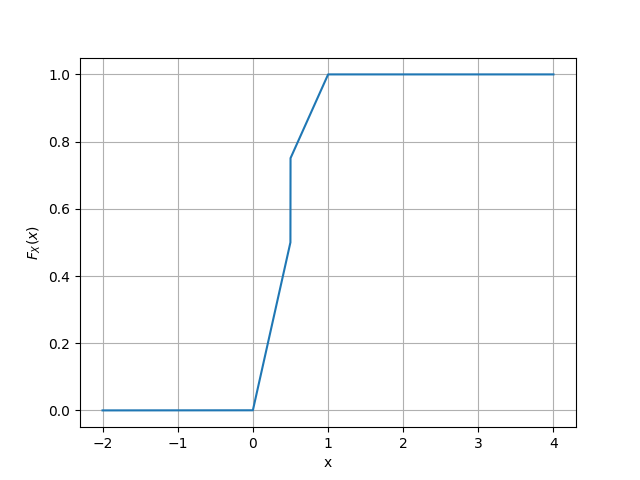
\includegraphics[width=8cm]{cdf_plot.png}
\caption{cdf of Random variable X}
\end{figure}

